\documentclass[letterpaper,journal]{IEEEtran}
\usepackage{amsmath,amsfonts}
\usepackage{algorithmic}
\usepackage{algorithm}
\usepackage{array}
\usepackage[caption=false,font=normalsize,labelfont=sf,textfont=sf]{subfig}
\usepackage{textcomp}
\usepackage{stfloats}
\usepackage{url}
\usepackage{verbatim}
\usepackage{graphicx}
\usepackage{cite}
\hyphenation{op-tical net-works semi-conduc-tor IEEE-Xplore}

\newcommand{\sysname}{\mbox{WISEConv}\xspace}
\usepackage{xspace}

\begin{document}

\title{\sysname: Worklist-driven Masked Convolution\\
for Onboard High-Speed Robotic Perception}

\author{Anonymous Authors% <-this % stops a space
\thanks{Manuscript received Month DD, YYYY.}}

% The paper headers
\markboth{IEEE Robotics and Automation Letters. Preprint Version.}%
{Author \MakeLowercase{\textit{et al.}}: \sysname: Worklist-driven Masked Convolution}

\maketitle

\begin{abstract}
Onboard robotic perception must sustain high update rates under tight compute
and power budgets. Masking policies from event increments, temporal frame
differences, and learned gates expose where computation is unnecessary, yet
existing execution paths do not convert this sparsity into commensurate latency
reduction. Tile skipping keeps the throughput of the dense pipeline but
recomputes inactive positions at tile granularity; gather-scatter selects active
positions exactly but loses throughput to feature materialization, irregular
access, and writeback. We present \sysname, a worklist-driven masked convolution
operator that drives tiled convolution from an active-output worklist rather than
a contiguous coordinate block, evaluating only active outputs while leaving the
per-position reduction and dense tensor layout intact. Selectivity thus becomes
exact without surrendering the regularity that gives the dense pipeline its
throughput. A single mask-space pass fuses output-mask propagation with per-tile
compaction and reuses coordinate metadata across compatible operators, keeping
construction cheap and infrequent. The worklist emits tile-local segments in
dense traversal order and decomposes work adaptively over the spatial and
reduction dimensions, sustaining near-dense throughput without input-patch
materialization or a global coordinate sort. Across various GPU platforms and
perception tasks, \sysname reduces full-model latency by 22--46\% relative to the
fastest competing path and per-frame energy by 28--60\% over dense convolution.
\end{abstract}

\begin{IEEEkeywords}
Computer architecture for robotic and automation, software, deep learning
methods, sparse convolution, embedded perception.
\end{IEEEkeywords}

\section{Introduction}
\label{sec:intro}

\IEEEPARstart{C}{onvolutional} networks support a broad range of onboard
robotic perception workloads, from high-rate motion and geometry estimation to
detection and pose estimation~\cite{fastdepth,nanoflownet,bisenet,densefusion}.
Their outputs feed online navigation, planning, and manipulation, so inference
latency limits how often downstream components can incorporate new
observations~\cite{contactgraspnet}. Meeting this latency demand is difficult
on board-level processors with constrained compute and power, because dense
convolution recomputes every spatial position on every invocation. Prior
systems avoid part of this work by deriving active masks from event-camera
increments, temporal frame differences, or learned spatial
gates~\cite{evconv,asyncsparse,deltacnn,dgnet,dynconv}. Although these policies
arise from different sensing modalities and tasks, they expose the same
operator-level problem: update selected positions on dense 2D feature grids
without computing inactive outputs.

Dense GPU convolution obtains high throughput from tiled, coordinate-driven
execution. Each tile enumerates a contiguous block of output coordinates; those
coordinates determine the input reads and output writes, while the reduction
over channels and kernel offsets follows a regular datapath. Neighboring
coordinates consequently share predictable memory access and data reuse. This
regularity, not merely the arithmetic count, is what a masked operator must
preserve.

Existing masked-convolution systems sacrifice one part of this structure or the
other. \emph{Tile skipping}~\cite{sbnet,skipconv,evconv,deltacnn} retains the
dense pipeline and suppresses a tile only when all its outputs are inactive, so
a single active position triggers computation for the entire tile.
\emph{Gather-scatter}~\cite{sai,dgnet,dynconv} instead extracts active
positions exactly, materializes their receptive fields, and scatters the
results back to the dense grid, trading regular execution for extraction,
irregular access, and writeback.

We characterize this trade-off along two axes (\S\ref{sec:bg:gap}):
\emph{throughput} (operations per second, bounded by the dense pipeline) and
\emph{useful-compute ratio} (the fraction of executed operations that produce
needed outputs). Tile skipping preserves throughput but sacrifices useful-compute
ratio; gather-scatter attains a useful-compute ratio near one but sacrifices
throughput and pays for extraction and writeback. Neither delivers both, so
upstream sparsity does not translate into proportional latency reduction. In our
sparsest workload, the masks render 84\% of the convolution work they govern
unnecessary. State-of-the-art tile skipping~\cite{deltacnn} still spends half of
its executed operations on unneeded outputs (a useful-compute ratio of 0.49) and
cuts latency by at most 41\%. Gather-scatter drives the useful-compute ratio close
to one, yet sustains only 9\% of tile skipping's throughput and runs 3.1$\times$
slower than dense convolution (\S\ref{sec:eval:latency}).

Our key insight is that position-level selectivity does not require abandoning
the dense convolution pipeline. A dense tile already derives its reads and
writes from output coordinates, so replacing its contiguous coordinate block
with an active-output worklist changes which outputs are evaluated without
changing the per-position reduction, the dense tensor layout, or the weight
layout. Selectivity then becomes exact by construction, pinning the
useful-compute ratio near one with no input-patch materialization. A high
useful-compute ratio alone does not yield latency reduction, however, since
gather-scatter also attains one and still loses. What a worklist operator must
additionally control is the cost of constructing the worklist and the throughput
at which it is consumed.

Two challenges follow. First, \emph{worklist-construction overhead}: constructing the worklist requires scanning the mask, and incurs cost that scales with the layer's spatial grid, not with the
active count or the channel widths, while the compute the worklist enables shrinks with
both the active count and the channel widths. 
Construction's share of latency therefore grows as activity falls
and channels thin, and accumulates per operator when every layer rebuilds.
Second, \emph{end-to-end worklist efficiency}: the worklist's order and length both
affect its consumption throughput, and sparsity worsens each.
An unordered worklist scatters the input neighborhoods that adjacent work
touches, lowering locality; its length falls below the dense grid and shifts with
layer and input, so no fixed tiling keeps the GPU full. Both effects sharpen
as activity falls.

We present \sysname, a \emph{Worklist-driven Masked Convolution} operator that
answers both challenges by co-designing worklist construction and convolution.
Construction is made cheap and infrequent: a single mask-space pass fuses
output-mask propagation with per-tile compaction, moving only mask and
coordinate metadata, and compatible operators propagate and reuse valid
coordinate metadata instead of reconstructing it. Consumption is made
dense-like: construction emits contiguous per-tile segments whose order follows
the dense tile traversal, giving compute tile-local spatial structure without a
global sort, and compute organizes parallel work adaptively over the spatial and
reduction dimensions according to device, layer shape, and activity, while each
selected position retains the regular reduction over channels and kernel
offsets.

This paper makes three contributions:
\begin{itemize}
  \item We characterize masked-convolution latency along two axes,
        useful-compute ratio and throughput, and show that tile skipping and
        gather-scatter each secure one at the other's expense, explaining the
        measured gap between required work and realized latency.

  \item We design \sysname, which fuses position-level selectivity into tiled
        dense convolution to secure both axes at once: an exact worklist pins
        the useful-compute ratio near one, fused mask-space construction with
        cross-operator metadata reuse bounds construction cost, and tile-local
        segment ordering with adaptive work decomposition keeps throughput close
        to the dense pipeline.

  \item We evaluate \sysname on four perception models spanning event
        increments, temporal frame differences, and learned spatial gating,
        across two Jetson embedded platforms and discrete laptop and desktop
        GPUs. \sysname reduces full-model latency relative to the fastest baseline by
        22--39\% on the Jetson platforms and 34--46\% on the discrete GPUs, and
        cuts per-frame energy over dense convolution by 28--60\% on the Jetson
        platforms.
\end{itemize}

\section{Background and Motivation}
\label{sec:background}

\subsection{Latency-Critical Onboard Perception}
\label{sec:bg:robotics}

Robotic perception runs inside an online sensing-to-action
loop~\cite{percsurvey,navsurvey}. Optical flow supplies motion estimates and
depth supplies obstacle geometry for navigation~\cite{nanoflownet,fastdepth},
segmentation supplies scene state for planning~\cite{bisenet}, and object pose
and grasp proposals guide manipulation~\cite{densefusion,contactgraspnet}. In
each case the inference output feeds a downstream component whose next decision
depends on the freshness of that estimate~\cite{pampc,perclatency}. Because
freshness is set by latency, a lower perception latency is always preferable:
where a task imposes a latency budget, a lower latency makes that budget easier
to meet; where none is fixed, it still lets the controller react to the
environment sooner~\cite{eventavoid,dronerace}. We therefore target latency
minimization rather than a preset deadline. Offloading to remote compute could
add capacity but is bounded by communication delay and
connectivity~\cite{cloudrobotics}, so we close the loop onboard under a limited
power and compute budget~\cite{onboardsensing}, minimizing end-to-end perception
latency on the target device.

One line of work is targeted to lower this latency by computing only the active region of each
frame, delivered as a spatial mask. The mask derives from event-camera
increments~\cite{asyncsparse,evconv}, temporal residuals between video
frames~\cite{cbinfer,skipconv,deltacnn}, or learned input-dependent
gates~\cite{sact,sai,dgnet,dynconv}. These sources differ in sensing modality
and policy, but all expose the same spatial sparsity on a dense 2D feature grid
for the convolution operator to exploit.

\subsection{Masked Convolution}
\label{sec:bg:masked}

Masked convolution keeps the dense tensors and arithmetic of a dense convolution
and restricts only which output coordinates it evaluates. It operates on an input
feature tensor $\mathbf{x}\in\mathbb{R}^{H_{in}\times W_{in}\times C_{in}}$, a
weight tensor $\mathbf{w}\in\mathbb{R}^{k\times k\times C_{in}\times C_{out}}$ of
kernel size $k$, and an output
$\mathbf{y}\in\mathbb{R}^{H_{out}\times W_{out}\times C_{out}}$ on a coordinate
grid $\mathcal{G}=\{1,\ldots,H_{out}W_{out}\}$, where each coordinate $p$ has a
$k\times k$ receptive field $\mathcal{N}(p)$ in $\mathbf{x}$. An upstream policy
marks the coordinates to compute in an output mask
$M_{out}\in\{0,1\}^{H_{out}\times W_{out}}$. Spatial gating predicts $M_{out}$
directly; event and temporal policies instead supply an input mask
$M_{in}\in\{0,1\}^{H_{in}\times W_{in}}$ whose active positions propagate their
influence along the receptive field, so $p$ stays active whenever any input in
$\mathcal{N}(p)$ is active,
\begin{equation}
  M_{out}[p] =
  \begin{cases}
    1, & \exists\, r\in\mathcal{N}(p)\ \text{s.t.}\ M_{in}[r]=1,\\
    0, & \text{otherwise.}
  \end{cases}
  \label{eq:mask}
\end{equation}
$M_{out}$ thus fixes which positions of $\mathbf{y}$ the operator updates, each
by aggregating $\mathbf{x}$ over $\mathcal{N}(p)$ with the weights $\mathbf{w}$.
The active ratio $\alpha = \|M_{out}\|_0 / |\mathcal{G}|$, the active fraction of
the grid, is the intrinsic sparsity the policy exposes.

An execution path realizes this mask over a compute set $\mathcal{C}$ bounded by
$\{p : M_{out}[p]=1\}\subseteq\mathcal{C}\subseteq\mathcal{G}$; for each
$p\in\mathcal{C}$ it computes
\begin{equation}
  \mathbf{y}[p] = \sum_{i=1}^{k^2}
  \mathbf{w}_i\,\mathbf{x}[\mathcal{N}_i(p)],
  \label{eq:conv}
\end{equation}
where $\mathcal{N}_i(p)$ is the $i$-th position in $\mathcal{N}(p)$ and
$\mathbf{w}_i\in\mathbb{R}^{C_{in}\times C_{out}}$ the corresponding weight
slice. The path must compute every active coordinate to avoid dropping a
requested output but may also compute inactive ones; dense convolution is the
extreme $\mathcal{C}=\mathcal{G}$. The policy alone fixes the accuracy and the
required work, while the choice of $\mathcal{C}$ is determined by the path.

\subsection{The Sparsity-to-Latency Gap}
\label{sec:bg:gap}

Existing systems execute a mask along one of two paths. \emph{Tile
skipping}~\cite{sbnet,skipconv,evconv} inherits the dense pipeline's tile-based
computation, skipping a tile only when all its coordinates are inactive and
otherwise computing the whole tile; DeltaCNN~\cite{deltacnn} fuses a selective
path into the kernel, taken when a tile is estimated to be mostly empty, cutting
wasted work while degrading throughput. \emph{Gather-scatter}~\cite{sai,dgnet}
instead extracts exactly the active coordinates, computes, and scatters them
back, removing the inactive arithmetic but adding extraction, irregular access,
and writeback overhead; DynConv~\cite{dynconv} adopts a model structure suited to
gather-scatter, where one gather feeds several consecutive layers before a single
scatter, amortizing that overhead.

We measure each path by two quantities. Its useful-compute ratio is the
fraction of computed coordinates that are active,
\begin{equation}
  \eta = \frac{\|M_{out}\|_0}{|\mathcal{C}|} \le 1.
  \label{eq:useful-ratio}
\end{equation}
Its throughput is the rate at which it processes issued FLOPs,
\begin{equation}
  T = \frac{2\,|\mathcal{C}|\,k^2 C_{in} C_{out}}{t},
  \label{eq:throughput}
\end{equation}
where $t$ is the per-frame latency and the leading factor of 2 counts each
multiply-accumulate as two FLOPs. For the required
$2\,\|M_{out}\|_0\,k^2 C_{in} C_{out}$ FLOPs, latency is set by the \textbf{effective
throughput} $T_{\mathrm{eff}} = \eta T$, the rate at which a path computes needed
outputs.

Figure~\ref{fig:gap} traces this on Jetson AGX Orin for the sparsest workload in our evaluation.
The policy marks 84.4\% of the convolution work unnecessary, and the sparse paths
discard it with negligible accuracy loss, so the remaining work sets a 9.6\,ms
latency floor (Fig.~\ref{fig:gap}a, dashed). Neither path approaches it: tile
skipping (DeltaCNN~\cite{deltacnn}) reaches 36.6\,ms, still 3.8$\times$ the floor, and gather-scatter, the
path DynConv is built around, runs at 194\,ms, far slower than dense convolution
itself. That is due to their low effective throughput from different causes. Tile skipping holds
throughput near half of dense but at a useful-compute ratio of only 0.49;
gather-scatter lifts the useful-compute ratio to one, yet extraction and data
movement collapse its throughput to 5\% of dense (Fig.~\ref{fig:gap}b). Neither
path efficiently converts the GPU's capability into effective throughput.

\begin{figure}[t]
  \centering
  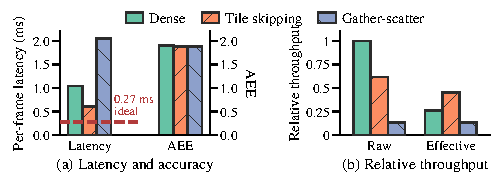
\includegraphics[width=\columnwidth]{figures/gap.pdf}
  \caption{Statistics of DynConv~\cite{dynconv}, a pose estimator
  with learned spatial gating, on the MPII human-pose dataset~\cite{mpii} and
  Jetson AGX Orin, comparing the native cuDNN path (Dense) against the two
  sparse paths.
  (a)~End-to-end average per-frame latency (left axis; the dashed line marks the
  dense latency scaled by the active ratio aggregated across layers) and PCKh
  accuracy (right axis; keypoints localized within half the head size). The
  sparse paths apply the same mask, so their accuracy coincides. (b)~Raw
  throughput $T$ and effective throughput $T_{\mathrm{eff}}$, aggregated across
  the model's convolution layers. The dense useful-compute ratio implies the
  active ratio set by DynConv's spatial gating ($\alpha\approx15.6\%$).}
  \label{fig:gap}
\end{figure}

\subsection{Relation to 3D Sparse Convolution}
\label{sec:bg:3d}

SpConv~v2 and TorchSparse++ target point clouds that are sparse by
representation, building coordinate maps over irregular voxel
coordinates~\cite{spconv2,torchsparsepp}. Our setting instead keeps dense 2D
tensors under a changing spatial mask, where the challenge is to skip inactive
outputs without turning a regular image-grid pipeline into an irregular one. We
therefore treat 3D sparse convolution as related infrastructure rather than a
primary baseline.

\section{\sysname Design}
\label{sec:design}

\subsection{Overview}
\label{sec:design:overview}

\sysname turns an upstream activity mask into the coordinate stream of a
tiled convolution. A layer receives a dense feature tensor $\mathbf{x}$ and
its input mask $M_{in}$. It produces the output values $\mathbf{y}$ requested
by the mask policy, the propagated output mask $M$, and a worklist $\mathbf{q}$
of active output coordinates. The operator separates this work into two stages
(Figure~\ref{fig:overview}):

\begin{enumerate}
  \item \textbf{Construction stage.} A mask-space kernel evaluates
        Eq.~\eqref{eq:mask}, writes $M$, and compacts its active coordinates
        into $\mathbf{q}$. It scans the output grid in spatial tiles, so each
        emitted segment retains the local traversal order of one tile.

  \item \textbf{Compute stage.} A tiled convolution kernel reads its output
        coordinates from $\mathbf{q}$ instead of enumerating a contiguous
        output region. For those coordinates, it preserves the regular
        reduction over input channels and kernel offsets used by dense
        convolution.
\end{enumerate}

This separation removes coordinate discovery from the convolution kernel's
critical path and establishes spatial structure before feature data are
accessed. Construction touches only masks and coordinates; compute retains
dense feature and weight tensors and executes one output for every worklist
entry. The following sections describe tiled construction and worklist-driven
compute.

% TODO: overview figure (double column)
\begin{figure*}[t]
  \centering
  \fbox{\parbox{0.9\textwidth}{\centering\vspace{2.5cm}%
    \textbf{[TODO]} \sysname overview. Left: dense input feature tensor and
    input mask. Middle: tiled construction emits the output mask and compact
    worklist segments. Right: worklist coordinates replace the contiguous
    coordinate source of tiled convolution; only active outputs are written.
    \vspace{2.5cm}}}
  \caption{The \sysname two-stage pipeline. Construction discovers active
  output coordinates and compacts each spatial tile into a worklist segment.
  Compute uses the resulting coordinates to drive a tiled convolution while
  retaining its regular channel and kernel reduction.}
  \label{fig:overview}
\end{figure*}

\subsection{Tiled Worklist Construction}
\label{sec:design:construct}

Construction must determine the active output set before convolution without
moving feature data or imposing a device-wide ordering pass. We partition the
output grid into contiguous construction tiles $T_1,\ldots,T_N$, each with a
fixed local traversal. For every position $p\in T_n$, the stage evaluates
Eq.~\eqref{eq:mask} and writes the result to $M[p]$. It then selects the active
positions within that tile:
\begin{equation}
  \mathcal{I}_n = \{j : M[T_n[j]]=1\},
  \label{eq:support}
\end{equation}
and emits their linear output coordinates in local traversal order:
\begin{equation}
  \mathbf{q}_n = (T_n[j])_{j\in\mathcal{I}_n}.
  \label{eq:pertile-gather}
\end{equation}

Tiles execute in parallel and reserve disjoint segments of the final
worklist. If $P$ denotes their reservation order, the resulting array is
\begin{equation}
  \mathbf{q} = [\mathbf{q}_{P_1};\ldots;\mathbf{q}_{P_N}],
  \qquad |\mathbf{q}|=\|M\|_0.
  \label{eq:worklist}
\end{equation}
Parallel scheduling may change the order of these segments, so \sysname does
not require or provide a global raster order. Its guarantee is tile-local:
every $\mathbf{q}_n$ contains coordinates from one contiguous output region
in that tile's traversal order. Generating this order during compaction avoids
a subsequent sort over the active set.

Algorithm~\ref{alg:construct} summarizes the stage. The fused pass visits
$H_{out}W_{out}$ output positions and examines at most $k^2$ input-mask
entries per position. Its $O(H_{out}W_{out}k^2)$ work is independent of
$C_{in}$ and $C_{out}$. We include construction in operator latency and measure
its cost directly in Section~\ref{sec:eval:overhead}.

\begin{algorithm}[t]
\caption{Tiled Worklist Construction}
\label{alg:construct}
\begin{algorithmic}[1]
\REQUIRE Construction tiles $T_1,\ldots,T_N$, input mask $M_{in}$
\ENSURE Worklist $\mathbf{q}$, output mask $M$
\FOR{each tile $T_n$ \textbf{in parallel}}
  \FOR{each position $p\in T_n$}
    \STATE $M[p]\leftarrow$ Eq.~\eqref{eq:mask}
  \ENDFOR
  \STATE $\mathbf{q}_n\leftarrow(T_n[j])_{j:M[T_n[j]]=1}$
  \STATE $b_n\leftarrow\operatorname{reserve}(|\mathbf{q}_n|)$
  \STATE $\mathbf{q}[b_n:b_n+|\mathbf{q}_n|]\leftarrow\mathbf{q}_n$
\ENDFOR
\end{algorithmic}
\end{algorithm}

\subsection{Worklist-Driven Convolution}
\label{sec:design:compute}

Implicit GEMM views convolution as a matrix product whose rows correspond to
output coordinates, columns to output channels, and reduction dimension to
input channels and kernel offsets. A dense kernel derives each row coordinate
from a contiguous output tile. \sysname instead loads those coordinates from
$\mathbf{q}$; the column and reduction dimensions remain regular.

The compute stage partitions the worklist into blocks of $B_M$ coordinates,
the output channels into blocks of $B_N$, and the reduction into steps of
$B_K$. Each compute tile first loads a coordinate block $\mathbf{q}'$. For
every reduction step, it derives input addresses from $\mathbf{q}'$, loads the
corresponding input and weight tiles, and accumulates their products. It then
writes the result to the dense output tensor at the same coordinates
(Algorithm~\ref{alg:compute}). The worklist schedules exactly the support of
$M$.

The input tile in Algorithm~\ref{alg:compute} is loaded directly from
$\mathbf{x}$ into the kernel's working storage; it is not materialized as a
separate global matrix. Construction order makes these loads less irregular
than an arbitrary active-coordinate list. Entries within each
$\mathbf{q}_n$ address nearby output positions and therefore nearby,
frequently overlapping input neighborhoods. A compute tile inherits this
locality when its coordinate block lies within a construction segment. It may
also cross segment boundaries, which affects locality but not correctness.
This limited guarantee lets compute exploit available spatial structure
without requiring globally sorted coordinates.

\begin{algorithm}[t]
\caption{Worklist-Driven Convolution}
\label{alg:compute}
\begin{algorithmic}[1]
\REQUIRE Worklist $\mathbf{q}$, input $\mathbf{x}$, weight $\mathbf{w}$
\ENSURE Output $\mathbf{y}$ at coordinates in $\mathbf{q}$
\FOR{each output tile $(b_m,b_n)$ \textbf{in parallel}}
  \STATE $\mathbf{q}'\leftarrow
    \mathbf{q}[(b_m{-}1)B_M:b_mB_M]$
  \STATE $\mathbf{a}\leftarrow\mathbf{0}_{B_M\times B_N}$
  \FOR{each reduction tile $r$ of width $B_K$}
    \STATE $\mathbf{x}'\leftarrow$ input tile addressed by
      $(\mathbf{q}',r)$
    \STATE $\mathbf{w}'\leftarrow$ weight tile addressed by $(b_n,r)$
    \STATE $\mathbf{a}\leftarrow\mathbf{a}+\mathbf{x}'\mathbf{w}'$
  \ENDFOR
  \STATE $\mathbf{y}[\mathbf{q}',b_n]\leftarrow\mathbf{a}$
\ENDFOR
\end{algorithmic}
\end{algorithm}

\section{Implementation}
\label{sec:impl}

We implement \sysname as a CUDA C++ extension for PyTorch. The current backend
executes FP32 tensors in channels-last layout and provides the mask-aware
operators required by the evaluated networks: convolution, transposed
convolution, pooling, pointwise activation, addition, concatenation, and
upsampling. A model-conversion pass replaces compatible PyTorch modules while
preserving the graph topology, convolution parameters, and learned weights.
The upstream application continues to generate masks.

The construction kernel assigns contiguous output positions to each warp. A
thread tests one receptive field and terminates once it finds an active input.
A warp ballot identifies active lanes, population counts give their local
ranks, and one atomic operation reserves a contiguous worklist segment for the
warp. Active lanes then write their coordinates in lane order. This realizes
the tile-local ordering in Section~\ref{sec:design:construct} without a
device-wide prefix scan or sorting pass. An identity $1\times1$ convolution
has the same input and output coordinate space; when its input already carries
compatible mask and worklist metadata, the operator reuses that worklist and
skips construction.

The compute kernel uses a persistent, tiled implicit-GEMM organization. It
keeps partial sums in registers and stages input and weight tiles through
shared memory. Supported architectures use asynchronous global-to-shared
copies, with a synchronous path for earlier GPUs. Split-$K$ exposes additional
parallel work when the active-coordinate dimension alone cannot occupy the
device. Transposed convolution follows the same output-driven organization,
but partitions output coordinates by stride phase so that each phase visits
only its valid kernel offsets.

Efficient scheduling depends jointly on the GPU, layer shape, and activity.
We therefore autotune the sparse tile shape and split-$K$ factor and cache the
choice by device, convolution parameters, activity level, and execution
policy. For layers whose state-update semantics permit dense evaluation, the
candidate set can also include a cuDNN path. A sparse-only policy isolates the
worklist-driven kernel, and the cache key distinguishes the two policies and
the requested determinism mode. Autotuning and one-time weight preparation
complete before the timed sequence described in Section~\ref{sec:eval:setup}.

For fixed input values, weights, and mask, \sysname evaluates
Eq.~\eqref{eq:conv} at every active output coordinate. Floating-point
reordering may produce small numerical differences from cuDNN, so we verify
active outputs with numerical tolerances rather than requiring bitwise
identity. This check separates backend correctness from the task-quality
effect of the fixed upstream mask policy.


% ---------------------------------------------------------------------------
% Remaining sections (to be written):
% \input{src/related}
\section{Evaluation}
\label{sec:eval}

\subsection{Experimental Setup}
\label{sec:eval:setup}

\paragraph{Platforms.}

We evaluate six GPU platforms. The four discrete GPUs are NVIDIA A100,
RTX~4090, RTX~3080, and RTX~4070 Laptop. The embedded platforms are Jetson
Xavier NX and AGX Orin; we also measure board energy on both. The discrete
platforms use PyTorch 2.1.2, CUDA 12.1, and cuDNN 8.9.2; both Jetson platforms
use PyTorch 2.1.0, CUDA 11.4, and cuDNN 8.6. All paths in the full workload
comparison use FP32 (SIMT) with TF32 disabled. Sensitivity studies additionally
evaluate FP16 (tensor core) on selected platforms. On each platform, all backends run under the same fixed clock and
power configuration.

\paragraph{Models, tasks, and mask sources.}
Our workloads (Table~\ref{tab:models}) span three vision tasks:
FireFlowNet~\cite{fireflownet} for event-based optical flow on
MVSEC~\cite{mvsec} with Ev-Conv~\cite{evconv} masks,
YOLOv8n and YOLOv8m~\cite{yolov8} for detection on MOT16~\cite{mot16} with
DeltaCNN's~\cite{deltacnn} temporal masks, and
DynConv~\cite{dynconv} for human pose on MPII~\cite{mpii} with learned spatial
gates. For every workload, calibration uses the training split, while all
reported results use a disjoint test split with the authors' released
weights~\cite{fireflownet,yolov8,dynconv}. Within each workload, we fix
inputs, weights, and upstream mask policy; every sparse path receives the same
layer masks, isolating the masked-convolution backend.

\begin{table}[htb]
\centering
\caption{Evaluation workloads.}
\label{tab:models}
\footnotesize
\setlength{\tabcolsep}{3pt}
\renewcommand{\arraystretch}{1.08}
\begin{tabular}{@{}
  >{\raggedright\arraybackslash}p{0.19\columnwidth}
  >{\centering\arraybackslash}p{0.22\columnwidth}
  >{\centering\arraybackslash}p{0.22\columnwidth}
  >{\centering\arraybackslash}p{0.22\columnwidth}@{}}
\hline
 & \textbf{FireFlowNet} \cite{fireflownet}
 & \textbf{YOLOv8n/m} \cite{yolov8}
 & \textbf{DynConv} \cite{dynconv} \\
\hline
Task & Optical flow & Detection & Human pose \\
Mask source & Ev-Conv~\cite{evconv} & DeltaCNN~\cite{deltacnn}
            & DynConv~\cite{dynconv} \\
Dataset & MVSEC~\cite{mvsec} & MOT16~\cite{mot16} & MPII~\cite{mpii} \\
Input size & $256{\times}256$ & $640{\times}640$ & $256{\times}256$ \\
Parameters & 0.056M & 3.16M~/~25.9M & 6.89M \\
Eval. samples & 196.8K & 2,575 & 2,958 \\
\hline
\end{tabular}
\end{table}

\paragraph{Baselines.}
We compare \sysname against three FP32 (SIMT) execution paths:
\textbf{Dense} (PyTorch/cuDNN~\cite{cudnn} with autotuning),
\textbf{Tile skipping} (DeltaCNN~\cite{deltacnn} for FireFlowNet and YOLO;
DynConv supplies output masks directly), and
\textbf{Gather-scatter} (DynConv's~\cite{dynconv} CUDA backend for pose;
MMCV's~\cite{mmcv} MaskedConv2d for FireFlowNet and YOLO).

\paragraph{Measurements.}

We measure per-frame full-model GPU latency over the complete evaluation
datasets. CUDA events bracket each frame's inference; after warm-up we run
three complete rounds and average per-frame latency across all frames and
rounds. The interval includes mask propagation, worklist construction, all
network operators, and output update; it excludes input transfer, offline
calibration, and one-time initialization. We report $\eta$, $T$, and
$T_{\mathrm{eff}}$ at the model level by accumulating required and issued
work across layers per frame (Eq.~\ref{eq:efficiency-framework}), then
averaging across frames. On the Jetson platforms, we integrate board-level
\texttt{VDD\_IN} power over each frame interval to obtain per-frame energy.
For accuracy, we follow the original protocols: AEE for optical
flow~\cite{evconv}, AP for detection~\cite{deltacnn}, and PCKh for
pose~\cite{dynconv}. MOT16 AP uses fixed pseudo-labels from a dense YOLO26x
teacher~\cite{yolo26} because ground-truth detections cover only the training
split.

\subsection{End-to-End Performance}
\label{sec:eval:end-to-end}

\begin{figure*}[htb]
  \centering
  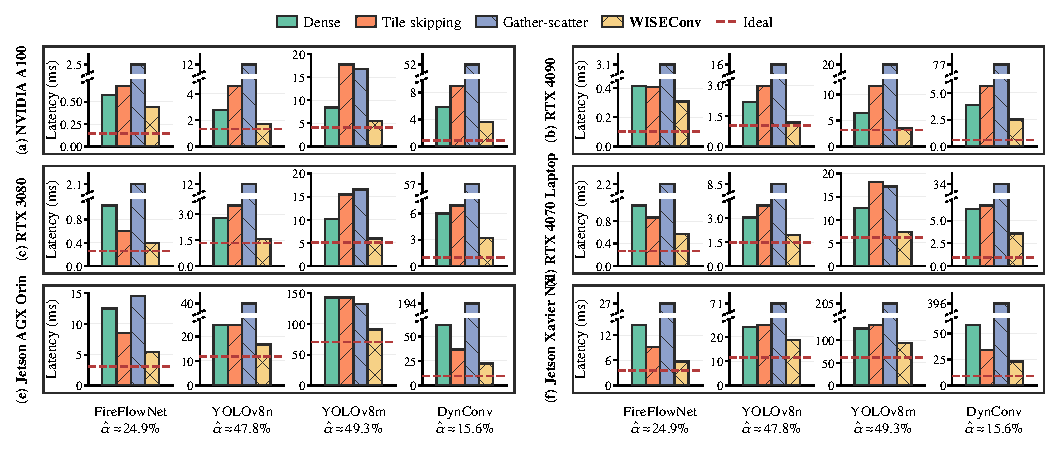
\includegraphics[width=\textwidth]{figures/e2e_latency.pdf}
  \caption{Full-model mean per-frame latency across GPU platforms. Each
  workload uses an independent y-axis. Labels report the model-level active
  ratio $\hat{\alpha}$, aggregated as described in
  \S\ref{sec:eval:setup} and averaged across evaluation sequences. Red dashed
  lines mark ideal proportional scaling, computed by applying each sequence's
  model-level active ratio to its dense latency before aggregation.}
  \Description{Grouped bar charts of full-model latency. Six platform panels
  each contain four workload groups comparing Dense, Tile skipping,
  Gather-scatter, and WISEConv. Selected workload groups use broken y-axes for
  a much slower gather-scatter path. Red dashed lines show the ideal
  proportional-scaling reference for each workload and platform, and workload
  labels report their aggregated active ratios.}
  \label{fig:e2e-latency}
\end{figure*}

\paragraph{Latency.}
\sysname is the fastest path in all 24
measured workload-platform pairs (Figure~\ref{fig:e2e-latency}). Relative to
the fastest evaluated competing path in each pair, it achieves a 1.57$\times$
geometric-mean speedup; individual-pair speedups range from 1.28$\times$ to
1.87$\times$, corresponding to 22.1--46.5\% lower latency. These gains persist
despite a more than two-order-of-magnitude span in absolute latency, from
0.309\,ms for FireFlowNet on RTX~4090 to 94.3\,ms for YOLOv8m on Xavier NX.

Unlike existing sparse paths, \sysname delivers uniform gains across workload
regimes. Dense is the fastest evaluated competing path in 15 of the 24
pairs, compared with eight for tile skipping and only one for gather-scatter;
sparsity magnitude alone does not determine where an existing sparse path
crosses the dense baseline.

\sysname's lead over the per-pair fastest competing path is narrower on the
embedded platforms (geometric mean 1.48$\times$ on Jetson vs.\ 1.62$\times$ on
discrete GPUs), though it remains fastest in all eight Jetson pairs, because
sparse paths are more effective on the narrower Jetson GPUs, leaving less
headroom.

\sysname also realizes more of the available sparsity headroom than every
competing path, running at 1.09--4.18$\times$ the ideal proportional-scaling
reference while the fastest competing path remains at 1.88--6.43$\times$.

\paragraph{Energy.}
\sysname is the lowest-energy path for every workload on both Jetson
platforms (Table~\ref{tab:e2e-energy}), reducing energy by
17.0--39.8\% relative to the lowest-energy competing path in each pair and by
28.5--72.6\% relative to dense execution.

% Generated by figures/plot_e2e.py from figures/e2e_stats.csv.
\begin{table}[b]
  \centering
  \caption{Per-frame board energy (J) on the Jetson platforms. Parentheses report each sparse path's change relative to Dense.}
  \label{tab:e2e-energy}
  \footnotesize
  \setlength{\tabcolsep}{1.2pt}
  \renewcommand{\arraystretch}{1.08}
  \begin{tabular}{@{}cc@{\hspace{4.0pt}}cccc@{}}
    \toprule
    \begin{tabular}[c]{@{}c@{}}GPU\end{tabular} & \begin{tabular}[c]{@{}c@{}}System\end{tabular} & \begin{tabular}[c]{@{}c@{}}FireFlowNet\end{tabular} & \begin{tabular}[c]{@{}c@{}}YOLOv8n\end{tabular} & \begin{tabular}[c]{@{}c@{}}YOLOv8m\end{tabular} & \begin{tabular}[c]{@{}c@{}}DynConv\end{tabular} \\
    \midrule
    \multirow{4}{*}{\rotatebox[origin=c]{90}{AGX Orin}} & Dense & 0.26 & 0.48 & 2.70 & 1.20 \\
     & Tile skip & 0.15\,(-43.8\%) & 0.44\,(-9.1\%) & 2.33\,(-13.7\%) & 0.67\,(-44.7\%) \\
     & Gather & 0.29\,(+9.5\%) & 0.70\,(+46.1\%) & 2.42\,(-10.4\%) & 2.37\,(+97.0\%) \\
     & \textbf{WISEConv} & \textbf{0.10}\,(-61.6\%) & \textbf{0.32}\,(-33.9\%) & \textbf{1.57}\,(-41.7\%) & \textbf{0.48}\,(-60.4\%) \\
    \midrule
    \multirow{4}{*}{\rotatebox[origin=c]{90}{Xavier NX}} & Dense & 0.28 & 0.49 & 2.58 & 1.08 \\
     & Tile skip & 0.13\,(-54.5\%) & 0.42\,(-13.8\%) & 2.27\,(-12.2\%) & 0.54\,(-50.4\%) \\
     & Gather & 0.33\,(+17.0\%) & 0.85\,(+75.8\%) & 3.18\,(+23.2\%) & 2.83\,(+160.9\%) \\
     & \textbf{WISEConv} & \textbf{0.08}\,(-72.6\%) & \textbf{0.35}\,(-28.5\%) & \textbf{1.78}\,(-31.1\%) & \textbf{0.34}\,(-68.5\%) \\
    \bottomrule
  \end{tabular}
\end{table}


\paragraph{Accuracy.}
\begin{figure}[htb]
  \centering
  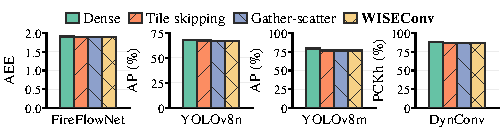
\includegraphics[width=\columnwidth]{figures/e2e_accuracy.pdf}
  \caption{Task accuracy on RTX~3080 under the evaluated upstream sparsity
  policies, measured by AEE~($\downarrow$), AP~($\uparrow$), and
  PCKh~($\uparrow$).}
  \Description{Four grouped bar charts compare Dense, Tile skipping,
  Gather-scatter, and WISEConv task accuracy. FireFlowNet reports average
  endpoint error, YOLOv8n and YOLOv8m report AP, and DynConv reports
  PCKh. The three sparse execution paths have closely matching task accuracy in
  every workload.}
  \label{fig:e2e-accuracy}
\end{figure}
\sysname's latency and energy gains do not alter accuracy:
AEE and PCKh match the other sparse paths at the reported precision, and
YOLOv8 AP differs by at most 0.5\% (Figure~\ref{fig:e2e-accuracy}).


\subsection{Microbenchmarks}
\label{sec:eval:microbenchmarks}

\begin{table}[!t]
  \centering
  \caption{WISEConv $\eta$ decomposition and worklist-length statistics
  on RTX~3080. The $n_{\mathcal{W}}$ percentiles are computed from worklist
  lengths pooled across all layers and frames.}
  \Description{A table reports eta construct, eta compute, eta, and the
  P10, P50, and P90 worklist lengths for FireFlowNet, YOLOv8n, YOLOv8m,
  and DynConv on RTX 3080. Worklist-length statistics are computed from samples
  pooled across all layers and frames.}
  \label{tab:worklist-efficiency}
  \footnotesize
  \setlength{\tabcolsep}{1.5pt}
  \renewcommand{\arraystretch}{1.12}
  \begin{tabular*}{\columnwidth}{@{\extracolsep{\fill}}l c c c r r r@{}}
    \hline
    \multirow{2}{*}{\textbf{Workload}} &
    \multirow{2}{*}{$\boldsymbol{\eta}_{\mathrm{construct}}$} &
    \multirow{2}{*}{$\boldsymbol{\eta}_{\mathrm{compute}}$} &
    \multirow{2}{*}{$\boldsymbol{\eta}$} &
    \multicolumn{3}{c}{$\boldsymbol{n}_{\mathcal{W}}$} \\
    \cline{5-7}
    & & & & \textbf{P10} & \textbf{P50} & \textbf{P90} \\
    \hline
    FireFlowNet & 99.9\% & 99.1\% & 98.9\% & $1{,}303$ & $15{,}083$ & $33{,}880$ \\
    YOLOv8n & 98.5\% & 97.7\% & 96.2\% & $77$ & $937$ & $5{,}937$ \\
    YOLOv8m & 98.7\% & 96.5\% & 95.2\% & $75$ & $840$ & $6{,}110$ \\
    DynConv & 100.0\% & 81.7\% & 81.7\% & $3$ & $43$ & $389$ \\
    \hline
  \end{tabular*}
\end{table}


\paragraph{Effective throughput.}
Under the same settings, we estimate
full-model throughput $T$ and effective throughput $\eta T$ on RTX~3080 and
AGX Orin (Figure~\ref{fig:effective-throughput}). \sysname sustains


30.7--87.2\% of Dense raw throughput on RTX~3080 and 58.6--83.5\% on AGX
Orin, the highest raw throughput among the sparse paths in every workload.
DeltaCNN's lower raw throughput reflects the impact of routing very sparse
tiles through its fused selective path~\cite{deltacnn}. The two YOLO workloads
lie at the upper end because their higher active ratios expose more parallelism
and amortize fixed costs. Combining throughput and useful-compute ratio,
\sysname reaches 1.52--1.78$\times$ the strongest competing effective
throughput on RTX~3080 and 1.45--1.65$\times$ on AGX Orin.

Table~\ref{tab:worklist-efficiency} localizes the remaining wasted work on
RTX~3080. Its $\eta_{\mathrm{construct}}$ stays at 98.5--100.0\%, while the
selected decompositions give $\eta_{\mathrm{compute}}=96.7$--$99.1\%$ for
FireFlowNet and the two YOLO workloads. DynConv instead has
$\eta_{\mathrm{compute}}=90.1\%$: its low
active ratio and small spatial grids yield exceptionally short worklists
(P10, P50, and P90 lengths of 3, 43, and 389), making final-tile padding
proportionally large. Because its inputs are temporally unrelated, DynConv uses
the same exact-length device policy without a temporal activity selector. Even
in this setting, this ratio
is substantially above tile skipping's 48.9\% on RTX~3080.
\begin{figure}[h]
  \centering
  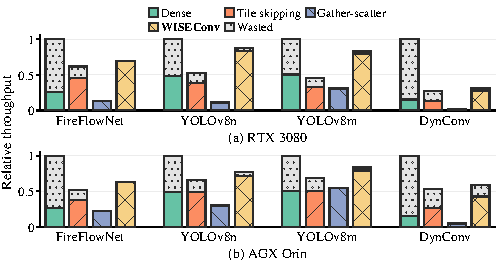
\includegraphics[width=\columnwidth]{figures/effective_throughput.pdf}
  \caption{Full-model effective throughput $\eta T$ and wasted throughput
  $(1-\eta)T$ on RTX~3080 and AGX Orin, normalized within each platform to
  Dense raw throughput.}
  \Description{Two vertically stacked platform panels compare Dense, Tile
  skipping, Gather-scatter, and WISEConv across four workloads. Each bar is
  divided into effective and wasted throughput, normalized to Dense raw
  throughput on the same platform.}
  \label{fig:effective-throughput}
\end{figure}

\begin{table}[!ht]
  \centering
  \caption{Full-model YOLOv8n cost decomposition in time (ms) and
  percentage on RTX~3080. Cost is classified into worklist construction
  (Cons.), convolution (Conv.), elementwise operators (Elem.), and other
  cost.}
  \Description{A table divides every YOLOv8n frame into low- and
  high-activity halves and compares full-model latency attributed to
  construction, convolution, elementwise, and other work for Dense, Tile
  skipping, Gather-scatter, and WISEConv. Construction is applicable only
  to WISEConv.}
  \label{tab:cost-decomposition}
  \footnotesize
  \setlength{\tabcolsep}{1.2pt}
  \renewcommand{\arraystretch}{1.15}
  \begin{tabular}{@{}c c c c c c c@{}}
    \hline
      & \textbf{System} & \textbf{Tot.} & \textbf{Cons.} &
      \textbf{Conv.} & \textbf{Elem.} & \textbf{Other} \\
    \hline
    \multirow{4}{*}{\rotatebox[origin=c]{90}{Low (40.7\%)}} & Dense & 2.79 & \textemdash{} & 2.54(91.2\%) & 0.14(5.0\%) & 0.10(3.7\%) \\
    & Tile skipping & 3.42 & \textemdash{} & 3.09(90.3\%) & 0.16(4.6\%) & 0.17(5.1\%) \\
    & Gather & 11.81 & \textemdash{} & 0.73(6.2\%) & 0.09(0.7\%) & 11.00(93.1\%) \\
    & \textbf{WISEConv} & 1.47 & 0.10(7.1\%) & 1.09(73.8\%) & 0.12(8.2\%) & 0.16(10.9\%) \\
    \hline
    \multirow{4}{*}{\rotatebox[origin=c]{90}{High (56.7\%)}} & Dense & 2.79 & \textemdash{} & 2.54(91.2\%) & 0.14(5.0\%) & 0.10(3.7\%) \\
    & Tile skipping & 3.59 & \textemdash{} & 3.25(90.4\%) & 0.17(4.7\%) & 0.18(4.9\%) \\
    & Gather & 11.82 & \textemdash{} & 0.83(7.0\%) & 0.09(0.8\%) & 10.90(92.2\%) \\
    & \textbf{WISEConv} & 1.69 & 0.11(6.2\%) & 1.29(76.3\%) & 0.13(7.7\%) & 0.17(9.8\%) \\
    \hline
  \end{tabular}
  \par\vspace{6pt}
  \noindent\parbox{\columnwidth}{\footnotesize\textit{Notes.} Low and High split
  all frames from the evaluated MOT16 test sequences at the median
  per-frame active ratio; their parenthesized labels report bin means.
  We obtain each stage time by multiplying its per-frame NSYS fraction
  by the corresponding CUDA-event latency from the end-to-end
  evaluation.}
\end{table}


\paragraph{Latency cost decomposition.}
We decompose full-model YOLOv8n latency by execution stage on RTX~3080 and AGX
Orin (Table~\ref{tab:cost-decomposition}). On the randomly sampled RTX~3080
frames, \sysname reduces the convolution share from 2.55 to 1.10\,ms while
adding only 0.10\,ms of construction; the corresponding sampled-row totals
are 2.79 and 1.49\,ms. On AGX Orin, construction accounts for 0.37\,ms, while convolution falls
from 22.61 to 13.41\,ms and the total falls from 25.09 to
17.07\,ms.

Gather-scatter has the lowest convolution time but \emph{Other} (extraction,
scatter, GEMM setup) accounts for 92\% of its total on RTX~3080, showing that
exact selection alone is insufficient without direct worklist consumption.

% Optional CUDA-level diagnostics are not a third required microbenchmark.
% If the two figures leave a concrete locality question, the useful diagnostic
% is whether tile-local worklists preserve dense-like cache behavior on the
% same real frames: collect L2 hit rate together with L2/DRAM traffic per
% required FLOP for Dense, WISEConv, and a sparse comparator.  L2 hit rate alone
% is insufficient because a path may issue fewer requests or transfer more
% bytes per useful output; report it only with traffic and the measured
% throughput, and keep the result as a small diagnostic rather than a
% standalone counter survey.

\paragraph{Memory overhead.}
Table~\ref{tab:memory} reports peak GPU memory. \sysname uses 10--12\% more
memory than tile skipping on the YOLO workloads, due to worklist buffers and
the partial-reduction workspace $\mathbf{Z}$; FireFlowNet's overhead is larger
(39\%) because its small model amplifies the fixed buffer cost. DynConv's gather-scatter backend reports the lowest footprint
because many of its layers do not maintain dense-layout intermediate tensors.

\begin{table}[htb]
  \centering
  \caption{Peak GPU memory (MiB) on RTX~3080.}
  \label{tab:memory}
  \footnotesize
  \setlength{\tabcolsep}{4pt}
  \renewcommand{\arraystretch}{1.08}
  \begin{tabular}{@{}lrrrr@{}}
    \hline
    \textbf{Workload} & \textbf{Dense} & \textbf{Tile skip} & \textbf{Gather-scatter} & \textbf{\sysname} \\
    \hline
    FireFlowNet & 65.9 & 174.1 & 166.0 & 242.1 \\
    YOLOv8n     & 164.9 & 253.2 & 238.7 & 279.7 \\
    YOLOv8m     & 195.1 & 854.3 & 825.7 & 956.2 \\
    DynConv     & 83.7 & 80.9 & 27.1 & 99.1 \\
    \hline
  \end{tabular}
\end{table}

\subsection{Ablation Study and Sensitivity Analysis}
\label{sec:eval:ablation-sensitivity}

\begin{table}[htb]
  \centering
  \caption{YOLOv8n component ablation on RTX~3080 and AGX~Orin.
  Times are milliseconds.}
  \Description{A table compares seven WISEConv design variants on RTX
  3080 and AGX Orin. Each platform reports useful-compute ratio,
  construction time, convolution time, and full-model latency.}
  \label{tab:ablation}
  \fontsize{7.0}{7.8}\selectfont
  \setlength{\tabcolsep}{0.7pt}
  \renewcommand{\arraystretch}{1.06}
  \begin{tabular*}{\columnwidth}{@{\extracolsep{\fill}}l c r r r c r r r@{}}
    \hline
    \multirow{2}{*}{\textbf{Variant}} &
    \multicolumn{4}{c}{\textbf{RTX 3080}} &
    \multicolumn{4}{c}{\textbf{AGX Orin}} \\
    \cline{2-5}\cline{6-9}
    & $\boldsymbol{\eta}$ & \textbf{Cons.} & \textbf{Conv.} & \textbf{Total}
    & $\boldsymbol{\eta}$ & \textbf{Cons.} & \textbf{Conv.} & \textbf{Total} \\
    \hline
    Atomic append   & 95.6\% & 0.169 & 1.241 & 1.862 & 93.1\% & 0.538 & 12.984 & 17.065 \\
    Global order    & 95.6\% & 0.265 & 1.180 & 1.897 & 93.1\% & 0.695 & 12.894 & 17.426 \\
    No reuse        & 97.0\% & 0.226 & 1.184 & 1.862 & 94.5\% & 0.648 & 12.739 & 17.112 \\
    DP only         & 95.5\% & 0.113 & 1.561 & 2.127 & 93.1\% & 0.359 & 13.940 & 17.942 \\
    No Hybrid       & 95.5\% & 0.113 & 1.227 & 1.793 & 93.1\% & 0.359 & 13.189 & 17.191 \\
    Sync exact selector & 95.5\% & 0.113 & 0.945 & 6.695 & 93.8\% & 0.352 & 10.328 & 23.787 \\
    \textbf{Ours}   & 95.5\% & 0.113 & 1.189 & 1.754 & 93.1\% & 0.359 & 12.994 & 16.996 \\
    \hline
  \end{tabular*}
\end{table}


Table~\ref{tab:ablation} isolates the construction and consumption choices on
YOLOv8n. On RTX~3080, Ours achieves 95.5\% useful-compute ratio at
1.754\,ms. Atomic append, Global order, and No reuse raise latency by
6.2\%, 8.2\%, and 6.2\%, respectively, exposing the cost of global
coordination and per-layer reconstruction. DP only is
21.3\% slower, whereas No Hybrid adds only 2.2\%.
Synchronizing the exact worklist length to the host costs 6.695\,ms
(3.82$\times$ Ours), confirming that host readback dominates any gain from
exact launch sizing.
On AGX~Orin the construction variants show smaller margins (0.4--2.5\%)
because convolution dominates the total. DP only adds 5.6\% and
Sync exact selector reaches 23.787\,ms (1.40$\times$): although its
convolution is faster (the host-selected tile count enables a tighter
decomposition), the per-operator synchronization adds 6.8\,ms of overhead
that erases the gain.

\begin{figure}[htb]
  \centering
  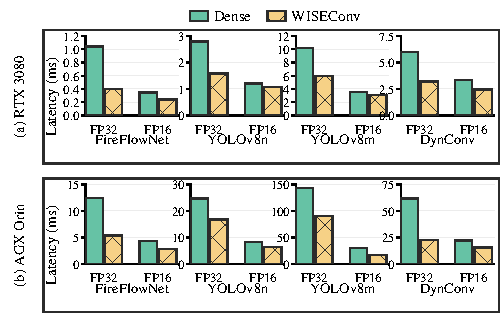
\includegraphics[width=\columnwidth]{figures/dtype_sensitivity.pdf}
  \caption{FP32 (SIMT) vs.\ FP16 (tensor core) full-model latency for
  Dense and \sysname across all four workloads. FP16 \sysname values for
  YOLOv8n and YOLOv8m are estimates from per-layer profiling.}
  \Description{Two panels (RTX 3080 and AGX Orin) each show four workload
  groups comparing Dense and WISEConv in FP32 and FP16.}
  \label{fig:dtype-sensitivity}
\end{figure}

\paragraph{Tensor core sensitivity.}
Figure~\ref{fig:dtype-sensitivity} compares FP32 and FP16 execution on
RTX~3080 and AGX~Orin. \sysname retains an end-to-end gain under tensor cores
on both platforms across all four workloads, although the gain narrows relative
to FP32 because tensor cores reduce the convolution time that \sysname saves
by skipping, shrinking the absolute saving while non-convolution costs
(construction, elementwise, mask processing) remain unchanged.

\begin{table}[!ht]
  \centering
  \caption{Stream-level batch sensitivity for full-model YOLOv8n on
  RTX~3080, decomposed by execution stage. All times are amortized
  ms/frame; parentheses report each stage's share of total latency.}
  \Description{A table compares Dense, Tile skipping, Gather-scatter,
  and WISEConv at batch sizes one, four, and eight. Each row gives
  amortized total latency per frame and its division among worklist
  construction, convolution, elementwise, and other work.}
  \label{tab:batch-cost-decomposition}
  \footnotesize
  \setlength{\tabcolsep}{1.0pt}
  \renewcommand{\arraystretch}{1.10}
  \begin{tabular}{@{}c@{\hspace{2pt}}l r c c c c@{}}
    \hline
    \textbf{B} & \textbf{System} & \textbf{Tot.} & \textbf{Cons.} &
    \textbf{Conv.} & \textbf{Elem.} & \textbf{Other} \\
    \hline
    \multirow{4}{*}{1} & Dense & 2.79 & \textemdash{} & 2.37(84.8\%) & 0.13(4.7\%) & 0.29(10.5\%) \\
    & Tile skip & 3.45 & \textemdash{} & 3.06(88.9\%) & 0.16(4.5\%) & 0.23(6.6\%) \\
    & Gather & 12.49 & \textemdash{} & 0.80(6.4\%) & 0.09(0.7\%) & 11.60(92.8\%) \\
    & \textbf{WISEConv} & 1.54 & 0.09(6.1\%) & 1.04(67.1\%) & 0.11(7.2\%) & 0.30(19.6\%) \\
    \hline
    \multirow{4}{*}{4} & Dense & 1.83 & \textemdash{} & 1.61(88.0\%) & 0.15(8.0\%) & 0.07(4.0\%) \\
    & Tile skip & 1.66 & \textemdash{} & 1.41(84.7\%) & 0.12(7.4\%) & 0.13(7.8\%) \\
    & Gather & 6.41 & \textemdash{} & 0.60(9.4\%) & 0.09(1.4\%) & 5.71(89.2\%) \\
    & \textbf{WISEConv} & 1.05 & 0.03(3.1\%) & 0.80(76.5\%) & 0.09(8.8\%) & 0.12(11.6\%) \\
    \hline
    \multirow{4}{*}{8} & Dense & 1.68 & \textemdash{} & 1.47(87.3\%) & 0.15(8.9\%) & 0.06(3.9\%) \\
    & Tile skip & 1.41 & \textemdash{} & 1.17(83.0\%) & 0.12(8.4\%) & 0.12(8.6\%) \\
    & Gather & 3.80 & \textemdash{} & 0.56(14.7\%) & 0.09(2.3\%) & 3.15(83.0\%) \\
    & \textbf{WISEConv} & 0.94 & 0.02(2.2\%) & 0.72(76.3\%) & 0.09(9.3\%) & 0.11(12.2\%) \\
    \hline
  \end{tabular}
  \par\vspace{5pt}
  \noindent\parbox{\columnwidth}{\scriptsize\textit{Notes.} Each $B$
  regroups the same 1,488 temporal transitions from eight disjoint
  MOT16-03 streams; every lane retains independent temporal state.
  Cons. is WISEConv worklist construction. Conv. is the backend's
  convolution path, and Elem. covers activation, residual, and
  concatenation work. Other contains remaining work and GPU timeline
  gaps; for Gather, this includes coordinate compaction, input-patch
  materialization, scatter, setup, and synchronization. Each stage
  scales its tensor-batch NSYS fraction by the corresponding formal
  CUDA-event batch latency before aggregation.}
\end{table}


\paragraph{Stream-level batching.}
Table~\ref{tab:batch-cost-decomposition} shows how stream-level batching
changes per-frame costs. At batch size~8, gather-scatter still spends 83.0\%
of its latency in \emph{Other}, whereas tile skipping becomes the fastest
competing path at batch sizes 4 and~8. Its launch grid is determined statically
from the input shape, so increasing the batch dimension adds independent tiles
from multiple temporal streams, consistent with DeltaCNN's observation for
high-end GPUs~\cite{deltacnn}. The effect is
concentrated in convolution: from batch size~1 to~8, tile skipping's per-frame
convolution cost falls 2.68$\times$, compared with 1.72$\times$ for \sysname.
\sysname remains fastest, but its lead narrows from 1.76$\times$ to
1.55$\times$. At batch size~1, adaptive decomposition substitutes for the
occupancy that batching would otherwise provide.

\subsection{Discussion}
\label{sec:eval:discussion}

\sysname consumes rather than generates masks, so its gains are conditional on
the upstream policy and its activity distribution; it guarantees coverage of
requested outputs but does not improve mask quality. The adaptive
decomposition is deployment-specific and must be recalibrated for a new model,
device, or mask workload; only offline policy interpolation can affect
performance, not coverage or correctness. The full workload comparison uses
FP32 (SIMT) because the evaluated
baselines~\cite{deltacnn,dynconv,mmcv} provide only FP32 paths. Extending
the worklist compute stage to tensor cores raises an open reduction problem:
split-$K$ partitions must accumulate FP32 partial sums and convert to FP16,
and for short worklists this overhead can outweigh the arithmetic savings.
The sensitivity study confirms that \sysname retains end-to-end gains under
FP16 tensor cores across all four workloads on both evaluated platforms.

% \section{Conclusion}
\label{sec:conclusion}

We presented \sysname, a masked-convolution runtime that replaces the dense
tiled pipeline's contiguous coordinate stream with an active-output worklist,
computing only positions an upstream mask marks active while retaining the dense
tensor layout and the regular per-position reduction. Construction completes in
a single mask-space pass and is reused across compatible operators; consumption
preserves tile-local ordering, bounds work with a device-resident worklist
length, and adapts its decomposition to input activity without host
synchronization. The four mechanisms are not independent additions: disabling
any one returns latency to either excessive construction cost or underloaded
consumption. Together they secure both useful-compute ratio and throughput,
converting upstream mask sparsity into end-to-end latency and energy reduction.
With \sysname, spatial masks become a reliable per-frame latency control for
real-time deployed perception systems.

% ---------------------------------------------------------------------------

\section*{Acknowledgments}
% TODO

\bibliographystyle{IEEEtran}
\bibliography{refs}

\end{document}
